% FreeDV-039 RADE presentation
% RADE presentation slides, intended for club level Ham presentation

\documentclass{beamer}

\usepackage{tikz}
\usetikzlibrary{calc,arrows,shapes,positioning,automata}
\usepackage{tkz-euclide}
\usepackage{graphicx}

\usetheme{CambridgeUS}

\title[RADE]{RADE - Machine Learning for Speech over HF Radio}
\institute[freedv.org]{freedv.org \and Supported by a grant from Amateur Radio Digital Communications}
\date[]{\today}

\begin{document}

% Tikz code used to support block diagrams
% credit: https://tex.stackexchange.com/questions/175969/block-diagrams-using-tikz

\tikzset{
block/.style = {draw, fill=white, rectangle, minimum height=3em, minimum width=3em},
tmp/.style  = {coordinate}, 
circ/.style= {draw, fill=white, circle, node distance=1cm, minimum size=0.6cm},
input/.style = {coordinate},
output/.style= {coordinate},
pinstyle/.style = {pin edge={to-,thin,black}}
}

% Title page frame
\begin{frame}
    \titlepage
\end{frame}

% Outline frame
\begin{frame}{Outline}
    \tableofcontents
\end{frame}

\section{Introduction}

\begin{frame}
\begin{description}
    \item[RADE] Radio Auto-encoder
\end{description}
\begin{itemize}
   \item Applying machine learning (ML) to send speech over HF radio 
   \item Combines traditional DSP and modern ML to encode and decode speech
   \item Connect a PC running RADE to your SSB radio
   \item 8 kHz audio bandwidth, high quality speech
   \item Works at low and high SNRs, handles multipath fading
\end{itemize}
\end{frame}

\begin{frame}{RADE Examples}
\begin{itemize}
\item  Texas to Australia, 25W, SNR 4 dB, deep fading \href{http://freedv.org/davids-freedv-update-september-2024/}
{\beamergotobutton{Link}}
\item 2000km Australian path, low and high SNR, barber pole fading \href{https://freedv.org/davids-freedv-update-june-2024}
{\beamergotobutton{Link}}
\end{itemize}
\end{frame}

\begin{frame}
RADE is an outcome of the FreeDV Project ...
\begin{itemize}
    \item Open source HF digital voice for amateur radio
    \item Since 2023, funded by an ARDC grant
    \item 6 person Project Leadership Team
    \item Financial sponsor is the Software Freedom Conservancy
    \item Project Goal: a voice mode competitive with SSB at high and low SNRs
\end{itemize}
\end{frame}

\section{Design Versus Training}

\begin{frame}

\begin{itemize}
	\item Previously, we would design a system
	\item Figure out all the signal processing steps
	\item With ML the emphasis is on training a neural network
	\item Consider an AM receiver example
	\item Lets build the Detector using machine learning
\end{itemize}

\begin{tikzpicture}[auto, node distance=3cm,>=triangle 45,x=1.0cm,y=1.0cm,align=center,text width=2cm]

% AM receiver block diagram

\node [input] (rinput) {};
\node [block, below of=rinput, node distance=1.25cm,text width=2cm] (bpf) {Band Pass Filter};
\node [block, right of=bpf] (detector) {(Diode) Detector};
\node [block, right of=detector] (lpf) {Low Pass Filter};
\node [output, below of=lpf, node distance=1.25cm,text width=2cm] (routput) {};

\draw [->] node[above,text width=2cm] {Input RF} (rinput) -- (bpf);
\draw [->] (bpf) -- (detector);
\draw [->] (detector) -- (lpf);
\draw [->] (lpf) -- (routput) node[below,text width=1.5cm] {Output Speech};
\end{tikzpicture}

\end{frame}

\begin{frame}
\begin{itemize}
	\item Start with an untrained neural network
	\item Collect some training material
	\item Many examples of input and desired output
	\item Adjust the network so it matches the desired output
\end{itemize}

% Detector training block diagram

\begin{tikzpicture}[auto, node distance=3cm,>=triangle 45,x=1.0cm,y=1.0cm,align=center,text width=2cm]

\node [input] (am_in) {};
\node [block, right of=am_in,node distance=2cm] (ml_det) {ML Detector};
\node [block, below of=ml_det,node distance=2cm] (adjust) {Adjust ML Detector};
\node [block, right of=adjust] (compare) {Compare};
\node [input, right of=compare,node distance=2cm] (det_out) {};

\draw [->] node[left,text width=1.5cm] {AM In} (am_in) -- (ml_det);
\draw [->] (ml_det) -| node[right] {ML Detector Out} (compare);
\draw [->] (det_out) -- node[right] {Detector Out} (compare);
\draw [->] (compare) -- (adjust);
\draw [->] (adjust) -- (ml_det);

\end{tikzpicture}

\end{frame}

\begin{frame}

\begin{figure}
\centering
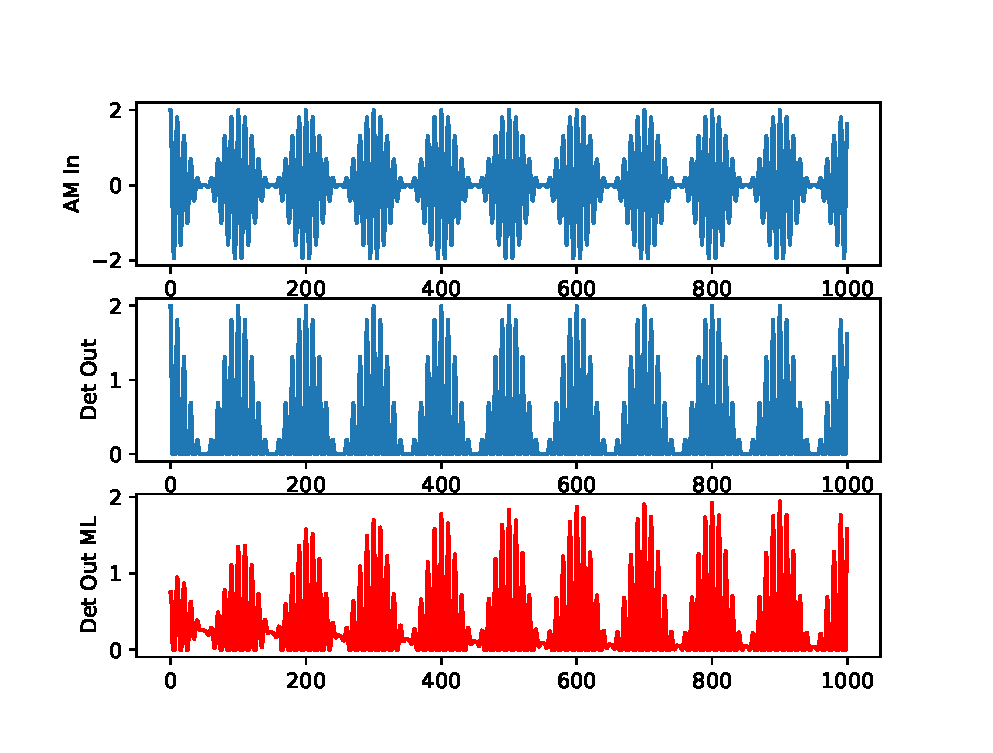
\includegraphics[width = 0.9\textwidth]{./ml_amdet}
\end{figure}
  
\end{frame}

\begin{frame}
\begin{itemize}
	\item Sometimes we don't know the best way to design something
	\item Real world problems are complex, perfect designs don't exist
	\item But we do have a good idea of what success looks (sounds) like
	\item So we just treat the system as a black box
	\item Show it examples of what we would like to see - and train
	\item ML has provided step changes in performance for many applications
	\item Including speech synthesis and compression
\end{itemize}
\end{frame}

\section{RADE Overview}

\begin{frame}
\begin{itemize}
	\item Jean-Marc Valin (and team) - compressing speech for Internet applications
    \item Idea: could it could be applied to noisy signal over radio channels?
    \item Jean-Marc developed a quick proof of concept
    \item We wrapped a modem around it, developed a practical HF voice system
    \item Hams around the world helped crowd sourced the testing
    \item Mooneer Salem integrated RADE with the FreeDV GUI application
\end{itemize}
\end{frame}

\begin{frame}
\begin{tikzpicture}[auto, node distance=3cm,>=triangle 45,x=1.0cm,y=1.0cm,align=center,text width=2cm]

% Classical DSP System

\node [input] (rinput1) {};
\node [block, below of=rinput1, node distance=1.25cm,text width=2cm] (feature_ext) {Feature Extraction};
\node [block, right of=feature_ext] (quant) {Quantisation};
\node [block, right of=quant] (fec_enc) {FEC Encode};
\node [block, right of=fec_enc] (mod1) {Modulator};
\node [block, below of=mod1, node distance=2cm] (channel1) {Radio Channel};
\node [block, below of=channel1, node distance=2cm] (demod1) {Demodulator};
\node [block, left of=demod1] (fec_dec) {FEC Decode};
\node [block, left of=fec_dec] (dequant) {De-Quant};
\node [block, left of=dequant] (synth) {Speech Synth};
\node [output, below of=synth, node distance=1.25cm,text width=2cm] (routput1) {};

\draw [->] node[above,text width=2cm] {Input Speech} (rinput1) -- (feature_ext);
\draw [->] (feature_ext) -- (quant);
\draw [->] (quant) -- (fec_enc);
\draw [->] (fec_enc) -- (mod1);
\draw [->] (mod1) -- (channel1);
\draw [->] (channel1) -- (demod1);
\draw [->] (demod1) -- (fec_dec);
\draw [->] (fec_dec) -- (dequant);
\draw [->] (dequant) -- (synth);
\draw [->] (synth) -- (routput1) node[below,text width=1.5cm] {Output Speech};
\end{tikzpicture}
\end{frame}

\begin{frame}
\begin{tikzpicture}[auto, node distance=3cm,>=triangle 45,x=1.0cm,y=1.0cm,align=center,text width=2cm]

% RADE System

\node [input] (rinput) {};
\node [block, below of=rinput, node distance=1.25cm,text width=2cm] (feature_ext) {Feature Extraction};
\node [block, right of=feature_ext] (rade_enc) {\emph{RADE} Encoder};
\node [block, right of=rade_enc,node distance=4cm] (ofdm_mod) {OFDM modulator};
\node [block, below of=ofdm_mod,node distance=2cm] (channel) {Radio Channel};
\node [block, below of=channel,node distance=2cm] (ofdm_demod) {OFDM demodulator};
\node [block, left of=ofdm_demod,node distance=4cm] (rade_dec) {\emph{RADE} Decoder};
\node [block, left of=rade_dec] (fargan) {Speech Synth};
\node [output, below of=fargan,node distance=1.25cm] (routput) {};

\draw [->] (rinput) node[above,text width=2cm] {Input Speech} -- (feature_ext);
\draw [->] (feature_ext) -- (rade_enc);
\draw [->] (rade_enc) -- node[above] {QAM Symbols} (ofdm_mod);
\draw [->] (ofdm_mod) -- (channel);
\draw [->] (channel) -- (ofdm_demod);
\draw [->] (ofdm_demod) -- node[above] {QAM Symbols} (rade_dec);
\draw [->] (rade_dec) -- (fargan);
\draw [->] (fargan) -- (routput) node[below,text width=1.5cm] {Output Speech};

\end{tikzpicture}
\end{frame}

\begin{frame}
\begin{itemize}
	\item Example of features - waterfall (aka spectrogram)
	\item A series of samples of the speech spectrum
	\item Encoder takes features and produces symbols we send over channel
	\item Decoder takes symbols and produces features
	\item Which are fed to a ML synthesiser to generate high quality speech
	\item Trained with 200 hours of speech, corrupted by noise and the HF channel
	\item Classical DSP modem wrapped around ML for synchronisation
\end{itemize}
\end{frame}

\begin{frame}

\begin{columns}
\begin{column}{0.5\textwidth}
  \begin{center}
  QPSK Constellation \\~\\
  \begin{tikzpicture}
  \draw (-2,-2.2) rectangle (2,2.2);
  \draw [fill] (-1,-1) circle (0.1);
  \draw [fill] (-1,1) circle (0.1);
  \draw [fill] (1,1) circle (0.1);
  \draw [fill] (1,-1) circle (0.1);
  \end{tikzpicture}
  \end{center}
\end{column}
\begin{column}{0.5\textwidth}  %%<--- here
  \begin{center}
  RADE Constellation \\~\\
  \scalebox{.6}{% Title: gl2ps_renderer figure
% Creator: GL2PS 1.4.2, (C) 1999-2020 C. Geuzaine
% For: Octave
% CreationDate: Fri Oct  4 09:19:32 2024
\setlength{\unitlength}{1pt}
\begin{picture}(0,0)
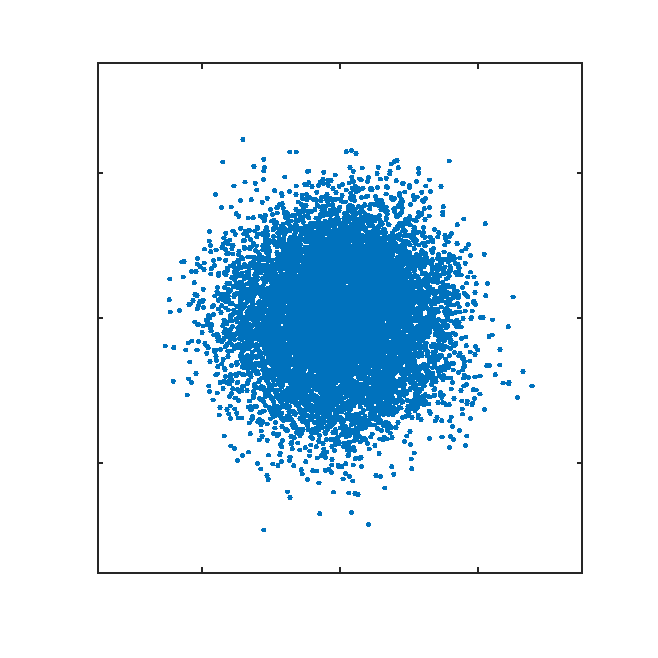
\includegraphics[scale=1]{model19_aux3_z_scatter-inc}
\end{picture}%
\begin{picture}(250,250)(0,0)
\fontsize{8}{0}\selectfont\put(74.1992,21.0029){\makebox(0,0)[t]{\textcolor[rgb]{0.15,0.15,0.15}{{-50}}}}
\fontsize{8}{0}\selectfont\put(129.375,21.0029){\makebox(0,0)[t]{\textcolor[rgb]{0.15,0.15,0.15}{{0}}}}
\fontsize{8}{0}\selectfont\put(184.551,21.0029){\makebox(0,0)[t]{\textcolor[rgb]{0.15,0.15,0.15}{{50}}}}
\fontsize{8}{0}\selectfont\put(28.1636,71.2979){\makebox(0,0)[r]{\textcolor[rgb]{0.15,0.15,0.15}{{-50}}}}
\fontsize{8}{0}\selectfont\put(28.1636,129.25){\makebox(0,0)[r]{\textcolor[rgb]{0.15,0.15,0.15}{{0}}}}
\fontsize{8}{0}\selectfont\put(28.1636,187.202){\makebox(0,0)[r]{\textcolor[rgb]{0.15,0.15,0.15}{{50}}}}
\fontsize{9}{0}\selectfont\put(129.375,241){\makebox(0,0)[b]{\textcolor[rgb]{0,0,0}{{Scatter}}}}
\end{picture}
}
  \end{center}
\end{column}
\end{columns}

\end{frame}

\section{Conclusion}

\begin{frame}{Conclusion}
\begin{itemize}
	\item Training versus Design
	\item RADE - Radio Autoencoder
	\item ML combined with classical DSP
	\item High quality speech over HF at low and high SNRs
	\item FreeDV GUI Application, sound card, SSB radio
	\item Supported by a grant from Amateur Radio Digital Communications
	\item Crowd sourced testing - thanks to many Hams around the world
	\item Developed by Hams for Hams
\end{itemize}

\end{frame}

\begin{frame}{Links}
\begin{description}
    \item[Download] freedv.org 
    \item[Help] freedv.org - mailing list, QSO finder chat, Discord chat
    \item[QSO Finder] qso.freedv.org \href{http://qso.freedv.org}{\beamergotobutton{Link}}
    \item[PSK Reporter] \href{https://pskreporter.info/pskmap?preset&callsign=ZZZZZ&what=all&mode=FREEDV&timerange=86400&mapCenter=17.5,-8,2.6}{\beamergotobutton{Link}}    
    \item[RADE Intro Doc] \href{https://github.com/drowe67/radae/blob/main/doc/rade_intro_waveform.pdf} {\beamergotobutton{Link}}
\end{description}
\end{frame} 

\end{document}
